%!TEX root = ../dissertation.tex
\chapter{Orthograph: Mapping coding nucleotide sequences to clusters of
orthologous genes}
\label{cha:orthograph}

\hyphenation{HaMStR pHMMs or-tho-lo-gy pa-ra-me-ters al-go-rith-mic}

\newpage

This chapter has been published in: \bibentry{Petersen2017}

\section{Background}\label{background}

Inferring the evolution of gene families, the phylogeny of species, and
tracing the biogeography of populations depend on reliable delineation
of orthologous genes and paralogous copies of them. While delineation
and identification of orthologous and paralogous genes has been firmly
established for studying genomic data (reviewed by \cite{Kristensen2011}
and benchmarked by \cite{Trachana2011}), few approaches are currently
available for assessing transcripts in the same manner (proposed by,
\emph{e.g.}, \cite{Ebersberger2009} and \cite{Schreiber2009}). Each of
these approaches exhibits, and suffers from, specific problems,
potentially leading to erroneous species and gene tree inference (see
below). We developed a novel software pipeline, called Orthograph, for
convenient, fast, and reliable identification of orthologous (and
paralogous) nucleotide or amino acid sequences, which resolves existing
algorithmic and software-technical issues. Orthograph builds on
previously proposed graph-based clustering algorithms, but extends them
without sacrificing accuracy or computational speed.

When comparing the gene repertoires of species, one of the first
analytical steps is the delineation of orthologous genes
(\emph{orthologs}), \emph{i.e.}, the identification of genes that
originated from a single gene in the last common ancestor of the
compared species. Each of the delineated orthologous groups (OGs) can
also include species- or lineage-specific gene copies
(\emph{inparalogs}), that evolved by gene duplication after the
evolutionary split of the ancestor into different species
\cite{Koonin2005}. Finally, horizontal gene transfer can give rise to
xenologous gene copies (\emph{xenologs}) from a single ancestral gene
\cite{Koonin2005}.

Two fundamentally different approaches to identify potential orthologs,
paralogs, and xenologs have been established: tree-based and graph-based
approaches. The benefit of graph-based approaches, which we will
subsequently focus on, is their computational efficiency and scalability
(for reviews and a comprehensive discussion of the benefits of the
different approaches, see \cite{Dutilh2007} or \cite{Kristensen2011}).
In general, graph-based approaches assessing gene orthology make use of
the genome-wide best reciprocal hit (BRH) criterion. It rests on the
assumption that orthologs in two genomes are more similar to each other
than to any other gene in the compared genomes, since they are direct
and exclusive descendants from a single ancestral gene
\cite{Altenhoff2012}.

Various graph-based approaches based on the BRH criterion have been
developed that \emph{de novo} infer orthology among genes and proteins
in the gene or protein sets of sequenced and annotated organisms, such
as OrthoMCL \cite{Li2003}, COCO-CL \cite{Jothi2006}, OrthoDB
\cite{Kriventseva2015}, InParanoid \cite{Sonnhammer2015}, OrthoFinder
\cite{Emms2015}, and OMA \cite{Altenhoff2015}. The reliability of these
methods critically depend on the fact that differential gene loss is the
exception and that gene or protein repertoires are complete. This means
that in order to apply a graph-based approach to infer gene orthology
among genomes, the organisms' gene or protein repertoire must be
reliably known. These methods are therefore not appropriate for
assessing orthology among nucleotide sequences in sequenced
transcriptomes, since transcript libraries contain only a subset of the
organisms' actual gene repertoire. The nucleotide sequence of a gene may
be missing in a given transcript library simply because the gene was not
(sufficiently highly) expressed at the time of RNA preservation. Given
that transcriptome sequencing represents an extremely valuable and
cost-efficient strategy to sample coding nucleotide sequences of a large
fraction of an organism's gene repertoire \cite{Misof2014}, several
graph-based approaches have been developed that are dedicated to
ortholog identification in transcript libraries.

A possible solution to the aforementioned problem in transcript
orthology assessment is to assign transcripts to OGs whose genealogical
relationships have already been reliably inferred, rather than to infer
orthology of these genes \emph{de novo} from the transcripts. Knowledge
of the genealogical relationships of genes can be derived from
comparative genomic analyses and may be retrievable from public
databases such as OrthoDB \cite{Kriventseva2015}. This approach has been
implemented in OrthoSelect \cite{Schreiber2009} and HaMStR
\cite{Ebersberger2009}. However, OrthoSelect does not implement the BRH
criterion, but a unidirectional search. OrthoSelect is thus prone to
false positives. HaMStR, on the other hand is more sophisticated since
it applies a BRH orthology prediction strategy. Specifically, HaMStR
uses profile hidden Markov models (pHMMs) that represent properties of
the aligned amino acid sequences of each known OG to search a transcript
library on the amino acid level for matches. All retrieved hits are then
searched against the entire set of proteins, \emph{i.e.}, the proteome
(also referred to as ``official gene set'') as reference gene set (RGS),
of each of the species of which amino acid sequences were used to
construct the pHMM. If this reciprocal search retrieves the same amino
acid sequence(s) that was (were) used in the construction of the pHMM, a
the respective transcript is mapped to the OG in question.

The algorithm of HaMStR is ``memoryless'', meaning that during
evaluation of the BRH criterion for a given OG, it does not consider
which transcripts have been assigned to other OGs. Since transcripts are
assigned to OGs on a per-OG basis without considering results from
evaluations for other OGs and keeping track of what transcripts have
already been assigned, it is possible that a given transcript is mapped
to more than one gene. This issue of redundant transcript assignments
can result in a misled inference of phylogenetic relationships, as has
been shown \cite{Struck2011,Kvist2013}, and can potentially compromise
downstream analyses. In HaMStR, it would be conceivable to prevent
redundant transcript assignment by implementing a record of previously
assigned transcripts. However, such a first-come-first-serve approach
cannot be justified: transcripts must be assigned to the OG that they
are most likely orthologous to, not to the OG that came first in the
search order. Since this serious issue cannot be solved using the HaMStR
algorithm, we developed Orthograph: a different algorithm that
circumvents redundant transcript assignments and instead maps
transcripts to the globally best matching OG.

To assess the sensitivity and accuracy of Orthograph, we tested whether
or not Orthograph a) reliably identifies orthologs, b) detects known
paralogs, and c) finds known isoforms or alternative transcripts. We
additionally searched 24 \emph{de novo}-sequenced transcript libraries
of apoid wasps for 5,561 orthologous genes to assess the computational
performance of Orthograph. Finally, we verified that Orthograph does not
map transcripts to more than one gene by re-analyzing a dataset that has
been processed with HaMStR. Our results demonstrate that Orthograph's
performance is on par with HaMStR's while not suffering from redundant
transcript assignment. Further, we emphasize the flexibility of
Orthograph and highlight features that are likely of particular interest
for a wide array of analyses in molecular evolutionary biology and in
	comparative genomics in particular.

\section{Implementation}\label{implementation}

The Orthograph software package is divided into three main tools that
handle (i) database management (manager), (ii) forward and reverse
searches (analyzer), and (iii) clustering of orthologous transcripts and
output (reporter). The separation into three distinct tools is a
deliberate design choice to address work environments where users do not
have full administrative privileges. This facilitates implementation in
a high-performance computing cluster setup where the administrator can
use the appropriate tool to manage the database, while users only need
to run the actual analysis tools. In addition, this design allows the
user to evaluate the alignment search results using different settings
(\emph{e.g.}, different alignment bit score thresholds to fine-tune and
optimize parameters) quickly without re-running the computationally
expensive searches.

Orthograph builds on the transcript orthology assessment strategy via
BRH suggested by \cite{Ebersberger2009}. In contrast to the
implementation of this strategy in HaMStR, Orthograph assigns a given
transcript to the \emph{globally} best matching OGs while making sure
that no transcript is assigned more than once. It additionally
identifies all transcripts (splice variants and inparalogs) present in
an assembled transcript library that are putatively homologous to a
given OG. The specific transcript orthology assignment algorithm is as
follows (Figure \ref{fig:orthograph-workflow} on page
\pageref{fig:orthograph-workflow}); note that steps 1 through 3 are only
required once since their output can be used for all subsequent
analyses:

\begin{enumerate}
\item
  The proteomes (``reference gene sets'', RGS) of reference species are
  used as input.
\item
  Orthologous genes from all reference proteomes are clustered to form
  orthologous groups (OGs). This information is provided from public
  databases or one's own orthology delineation in the RGS.
\item
  For each OG, the amino acid sequences are aligned and the multiple
  sequence alignment (MSA) is used to construct a profile HMM.
\item
  These pHMMs are used to search the transcript sequences on the amino
  acid level for candidate homologs.
\item
  Search results are stored in a relational database.
\item
  For each pHMM search hit, the target amino acid sequence section
  matching the pHMM is used as a query to search in a database that
  includes all genes from the RGS (including the genes that form OGs) on
  the amino acid level.
\item
  The results of the reverse search are also stored in the relational
  database.
\item
  After all forward and reverse searches have completed, the clustering
  of BRH pairs takes place: search results from all forward searches are
  sorted by descending alignment bit score. For each forward alignment
  search result, the corresponding reverse alignment search results are
  sorted by descending alignment bit score as well. They are evaluated
  in order of descending alignment bit score for the forward search
  results, starting with the highest alignment bit score.
\item
  If the best reverse search hit of a given transcript is part of the OG
  that the pHMM for the forward search is based on (\emph{i.e.}, the BRH
  criterion is fulfilled), the target transcript is assigned to the OG.
  The target transcript section is marked so that it cannot be assigned
  again. Each entry in the database is evaluated in this manner.
\end{enumerate}

Orthograph performs several post-processing steps on transcripts
assigned to OGs. By aligning the transcript fulfilling the BRH criterion
to the most similar orthologous amino acid sequence of a reference
species using Exonerate \cite{Slater2005}, it infers a
frameshift-corrected open reading frame (ORF). Orthograph allows to
extend the ORF beyond the pHMM alignment sequence section for which the
BRH criterion was fulfilled while making sure that the orthologous
region is covered by a user-defined percentage of the ORF length.
Subsequently, it provides both the amino acid sequence and the exactly
corresponding frameshift-corrected nucleotide sequence of a given
transcript. Additionally, Orthograph can concatenate transcripts of a
given OG to simplify downstream analyses (\emph{e.g.}, phylogenomic
investigations). In all above analysis steps, the user can fine-tune all
relevant search and evaluation parameters using configuration files for
clarity, documentation, and reproducibility.

\begin{figure}[t]
\begin{center}
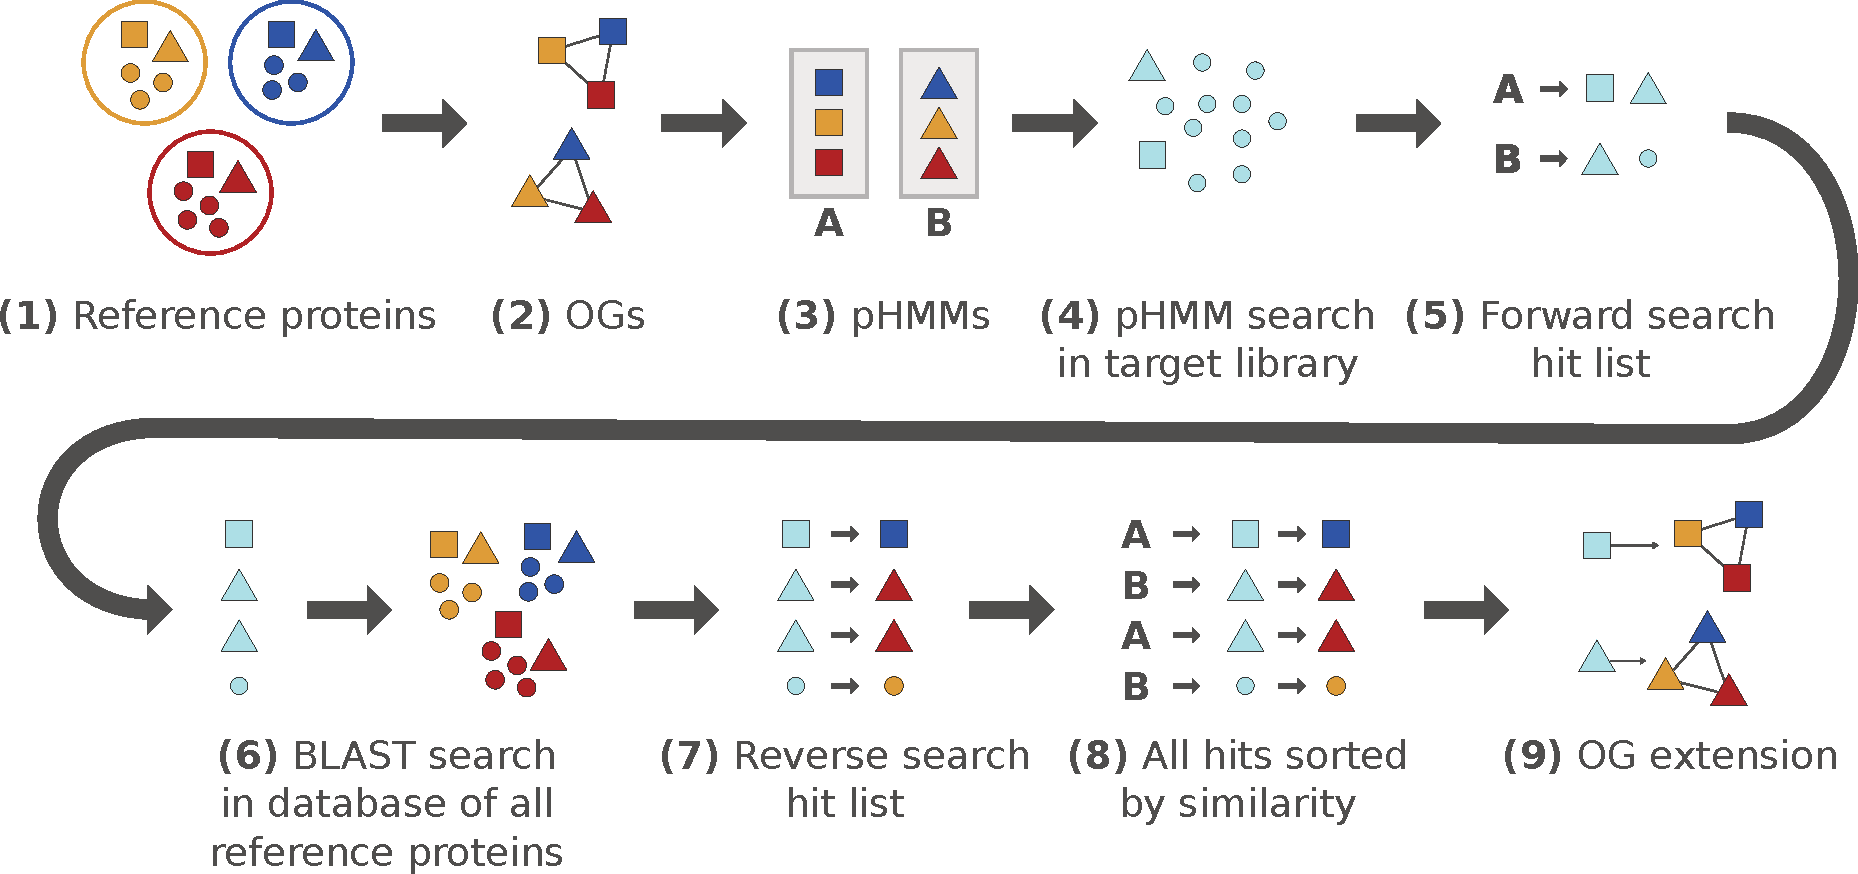
\includegraphics[width=\textwidth]{orthograph-workflow}
\caption[Orthograph workflow]{Orthograph workflow. From a set of
reference proteins (1), the proteins are clustered to form orthologous groups
(OGs) (2). These OGs are aligned to construct profile hidden Markov models
(pHMMs) (3). The pHMMs are used to search for candidate orthologs in the
target library (4). Each of the obtained hit amino acid sequences (5) is used
as a query for a BLAST search in a database comprising all reference proteins
(including the ones forming OGs) (6). Search results from both forward and
reverse searches (7) are collated and sorted by bit score, with the reverse
search result order being subordinated to the forward result order (8). This
list is evaluated in descending order: if the reverse search hit a protein
that is part of the OG used for the forward search, the candidate ortholog is
mapped to the OG (9).}
\label{fig:orthograph-workflow}
\end{center}
\end{figure}

Orthograph has been developed with user friendliness in mind. As a
result, it is easy to install and runs on any Unix/Linux system
(including OS X) that provides its dependencies (see Materials and
Methods). The generation of custom-tailored ortholog sets, \emph{e.g.},
from public databases is facilitated by its ability to parse simple
tab-delimited tables. Input from public databases such as OrthoDB is
easily formatted accordingly using standard UNIX or spreadsheet tools.
In addition, the Orthograph package contains helper scripts that
simplify the preparation of RGS sequence files for custom-made ortholog
sets as well as summarize results for multiple analyses, \emph{e.g.},
different species or using different settings.

When designing a custom ortholog set, users should pay close attention
to the taxon sampling. Genes that occur in at least two species in each
OG are recommended so that the resulting pHMMs are more informative than
when based on single sequences only. In terms of OG number, there is no
lower or upper bound since the selection depends on the research
question. Orthograph runtime increases linearly with each additional OG.

Detailed methods, data sources as well as system requirements are listed
in the Supplemental Material (Figures S1-S5, Tables S1-S3).

\section{Results and discussion}\label{results-and-discussion}

\subsection{Sensitivity and accuracy when searching for single-copy
orthologs}\label{sensitivity-and-accuracy-when-searching-for-single-copy-orthologs}

To assess the sensitivity and accuracy of Orthograph, we employed it to
identify genes of known orthology in the RGS of the honeybee,
\species{Apis mellifera} (15,314 genes, \cite{Honeybee2006}), and
Jerdon's jumping ant, \species{Harpegnathos saltator} (18,564 genes,
\cite{Bonasio2010}).  Specifically, we searched the RGS for 4,625
protein-coding genes provided by OrthoDB 5 \cite{Waterhouse2011a} as
being single-copy across four species of Hymenoptera (\species{Apis
mellifera} \cite{Honeybee2006}, \species{Camponotus floridanus}
\cite{Bonasio2010}, \species{Harpegnathos saltator} \cite{Bonasio2010},
\species{Nasonia vitripennis} \cite{Werren2010}) and the outgroup beetle
\species{Tribolium castaneum}
\cite{TriboliumGenomeSequencingConsortium2008} (download URLs are listed
in the Supplemental Material, Table S3). Note that we removed all
entries of the respective taxon whose RGS we analyzed for assessing the
sensitivity and accuracy of Orthograph from this ortholog set (resulting
in two sets: one without entries from \species{A. mellifera}, and one
without entries from \species{H.  saltator}). Of the 4,625
protein-coding genes that we searched for, Orthograph identified 4,582
(99.07 \%) in the RGS of \species{A. mellifera} and 4,590 (99.24 \%) in
the RGS of \species{H. saltator} (Table \ref{tab:orthograph-tests} on
page \pageref{tab:orthograph-tests}). In the case of \species{A.
mellifera}, five proteins were assigned to other OGs than they were
assigned by OrthoDB. We found a similar result for three proteins of the
RGS of \species{H. saltator}. Visual inspection of these proteins
suggested that the orthology assignment of these proteins in the OrthoDB
database is not correct (for an in-depth assessment and discussion of an
example see Supplemental Material, Figure S5). The low fraction (less
than 1 \%) of non-recalled genes were caused by a comparable effect
(Figure S5).  Thus, the sensitivity (true positive rate), defined as the
ratio of true positives to true positives plus false negatives, was
0.9896 for the \species{A. mellifera} RGS and 0.9918 for the \species{H.
saltator} RGS. The accuracy, defined as the ratio of true positives plus
true negatives to the total number of genes in the RGS, was 0.9965 for
the \species{A. mellifera} RGS and 0.9978 for the \species{H. saltator}
RGS.

For comparison, HaMStR v13.2.3 was run on the same datasets with
comparable parameters. HaMStR identified 4,589 genes (99.22 \%) in the
RGS of \species{A. mellifera} (1 false positive) and 4,573 genes (98.88
\%) in the RGS of \species{H. saltator} (2 false positives). This
results in a sensitivity of 0.992 in the \species{A. mellifera} RGS and
of 0.9883 in the \species{H. saltator} RGS, and an accuracy of 0.9975 in
the \species{A.  mellifera} RGS and of 0.9969 in the \species{H.
saltator} RGS.

The input data on ortholog relations were retrieved from OrthoDB which
contains OG information inferred in a purely automated fashion
\cite{Waterhouse2011a}. OrthoDB has been attested low numbers of false
positives and spurious assignments \cite{Trachana2011}; the proportion
of less than 1 \% of the genes that were recalled wrongly by Orthograph
are in line with these benchmarks. Orthograph and HaMStR perform roughly
equally in accuracy and sensitivity when it comes to identifying
single-copy orthologs.


% Please add the following required packages to the document preamble:
% \usepackage{booktabs}
\begin{sidewaystable}[h!]
\caption[Orthograph performance compared to
HaMStR \citep{Ebersberger2009}]{Results from the tests that compare
Orthograph performance to HaMStR \citep{Ebersberger2009}.  Sensitivity
is defined as the ratio of true positives (TP) to TP plus false
negatives (FN). Accuracy is defined as the ratio of TP plus true
negatives (TN) to the total number of genes in the official gene set
(OGS). FP, false positives. Note that the results are meant to
demonstrate equality in performance despite algorithmic
differences.}\label{tab:orthograph-tests}
\begin{tabular}{@{}llrlrrrrrrr@{}}
\toprule
Software   & Test        & Genes  & Species                & OGS       & Found  & TP    & FP & FN & Sens.       & Acc.  \\
\midrule
Orthograph & single-copy & 4,625  & \textit{A. mellifera}  & 15,314    & 4,582  & 4,577 & 5  & 48 & 0.990       & 0.996 \\
Orthograph & single-copy & 4,625  & \textit{H. saltator}   & 18,564    & 4,590  & 4,587 & 3  & 38 & 0.992       & 0.997 \\
HaMStR     & single-copy & 4,625  & \textit{A. mellifera}  & 15,314    & 4,589  & 4,588 & 3  & 39 & 0.992       & 0.997 \\
HaMStR     & single-copy & 4,625  & \textit{H. saltator}   & 18,564    & 4,573  & 4,571 & 2  & 54 & 0.988       & 0.996 \\
Orthograph & isoforms    & 8      & \textit{C. floridanus} & 17,064    & 7      & 7     & 0  & 1  & 0.875       & 0.999 \\
HaMStR     & isoforms    & 8      & \textit{C. floridanus} & 17,064    & 7      & 7     & 0  & 1  & 0.875       & 0.999 \\
Orthograph & inparalogs  & 647    & \textit{A. cephalotes} & 18,093    & 583    & 583   & 0  & 6  & 0.901       & 0.996 \\
\bottomrule
\end{tabular}
\end{sidewaystable}

\subsection{Identification of splice variants or
isoforms}\label{identification-of-splice-variants-or-isoforms}

We used Orthograph to assess orthologous amino acid sequences including
isoforms in the RGS of the Florida carpenter ant, \species{Camponotus
floridanus}, a species whose genes and corresponding proteins are part
of the ortholog set analyzed before (see above). In the \species{C.
floridanus} RGS, eight genes that are part of the ortholog set each
encode an alternative isoform. Orthograph readily assigned the
alternative isoforms of seven of these genes to the correct OGs. In the
remaining gene, however, the amino acid sequence of the isoform that
Orthograph could not find was very short (46 amino acids) in length.
Only 21 of the 46 amino acid sites can be well aligned to the OG and
were identified as BRH. It is possible that amino acid sequences that
are significantly shorter than the majority of the OG are scored poorly
by the pHMM search and/or the subsequent reverse search so that they
eventually do not fulfill the BRH criterion and are not recognized by
Orthograph.

HaMStR, in comparison, also identified all isoforms of seven of the
eight genes correctly. However, it reports them as co-orthologs.
Strictly speaking, this term is only correct when, while searching for
single-copy orthologs, one or more copies of the same gene are
identified. Orthograph, in addition to reporting, provides tabular
output with alignment coordinates, HMM alignment bit scores and e-values
for further statistical analyses.

While it would be highly desirable for users to also obtain information
on the occurrence of different isoforms (or alternative transcripts on
the transcriptional level) in different species, alternative transcripts
are difficult to distinguish from transcripts of inparalogs or from
transcript assembly artifacts without additional information, for
example on the genealogy of the species, whose transcript libraries have
been investigated, and/or on the transcript's expression level. However,
Orthograph provides tabular output files that can facilitate
corresponding downstream analyses. Specifically, the Orthograph output
files inform about a) what transcripts form BRHs with ortholog groups
and b) what transcripts assigned by Orthograph to the same ortholog
group overlap (\emph{i.e.}, partially refer to the same coding sequence)
and could thus represent alternative transcripts (or assembly
artifacts).

\subsubsection{Protein isoforms and splice variants in the reference
ortholog set can lead to systematic errors and false
positives}\label{protein-isoforms-and-splice-variants-in-the-reference-ortholog-set-can-lead-to-systematic-errors-and-false-positives}

The presence of isoforms and splice variants in an RGS dataset can lead
to wrong clustering to OGs and/or false negatives (discarded sequences
that should have been mapped elsewhere). Because it is impossible to
know in advance which isoform of a gene or transcribed gene is present
in a given transcript library, it is likely that a BRH search will fail
if more than one highly similar amino acid sequence are present in the
reference RGSs. This occurs because the best reverse search hit of a
candidate ortholog against the database comprising all proteins in an
RGS may return an isoform of the protein that was not used in the pHMM,
leading to a failure to fulfill the BRH criterion. Therefore, isoforms
should either be removed from RGS databases prior to using them in
Orthograph (or in any reference-based orthology prediction tool, for
that matter), or the OGs should be extended to also include the
isoforms.

\subsection{Identification of
inparalogs}\label{identification-of-inparalogs}

In order to demonstrate Orthograph's capabilities to detect inparalogous
gene copies, we used it to assess genes that are known to have
inparalogous copies in the RGS of the leafcutter ant, \species{Atta
cephalotes} \cite{Suen2011}. Specifically, we retrieved an ortholog set
from OrthoDB 5 comprising 301 OGs that contain genes that are known to
be single copy in the genomes of \species{A. mellifera}, \species{C.
floridanus}, \species{H. saltator}, \species{N. vitripennis}, and
\species{T.  castaneum}, but are multi-copy genes in \species{A.
cephalotes}. These 301 OGs include altogether 647 single-copy and
multi-copy genes from \species{A. cephalotes}: 273 are duplicated, 18
are triplicated, seven have four copies, two have six copies and one has
seven copies. Orthograph readily assigned 583 of the 647 multi-copy
genes to the correct OG (90.1 \%). Two of the 301 OGs were not assigned,
one of which contained four, the other contained two gene copies. In
both cases, the genes from \species{A. cephalotes} were much shorter
than the remaining genes in the OG (18 \% resp. 19 \% of the average
amino acid sequence length), possibly leading to the respective
transcripts failing to fulfil the BRH criterion in the reverse search
step due to an insufficient alignment length. These edge cases again
highlight the importance of high-quality genome sequencing and
annotation efforts, as they provide the basis for many downstream
analyses, including full-length gene sequences for reference-based
orthology assessment.

\subsection{Non-redundant mapping of
transcripts}\label{non-redundant-mapping-of-transcripts}

In order to test whether Orthograph indeed does not assign transcripts
to more than one OG, we re-analyzed the dataset published by
\cite{Struck2014}, who used HaMStR version 8 \cite{Ebersberger2009}.
Orthograph assigned transcripts to 1,253 OGs, the same number as
obtained by \cite{Struck2014}. However, Orthograph found transcripts of
the analyzed genes in, on average, slightly more taxa (Orthograph:
28.079, \cite{Struck2014}: 26.699). None of the transcripts was assigned
to more than one OG. In the dataset published by \cite{Struck2014}, 274
transcripts were assigned redundantly, however the orthologous regions
were not overlapping. As \cite{Struck2014} removed a total of 1.3 \% of
their sequences from the dataset due to redundantly assigned
transcripts, Orthograph yielded 1.4 \% more taxa per gene, leading to a
denser data matrix for downstream (phylogenetic) analyses.

\subsection{Computational performance of
Orthograph}\label{computational-performance-of-orthograph}

To demonstrate the computational performance of Orthograph, we searched
24 apoid wasp transcriptome assemblies for 5,561 selected OGs (sequence
data are deposited at NCBI GenBank; accession numbers are listed in
Additional file 2). The analysis time when using a single thread
increases linearly with total transcriptome assembly length (Spearman
rank correlation, $S = 326$, $p \ll 0.001$, Supplemental Material,
Figure S3). Single-threaded analysis time also increases with the number
of assembled transcripts, showing a linear trend, but no significant
correlation (Spearman rank correlation, $S = 1,430$, $p = 0.069$).

Given that next-generation RNAseq datasets tend to be large and current
comparative genomic investigations analyze hundreds, if not thousands of
genes (\emph{e.g.}, \cite{Misof2014}, \cite{Jarvis2014}, the 1000 plants
initiative (\url{https://sites.google.com/a/ualberta.ca/onekp/})), with
a linear runtime increase Orthograph does not pose a time bottleneck for
current and future large-scale studies such as the numerous
group-specific subprojects of the 1KITE consortium
(\url{http://1kite.org/subprojects.html}). For employment in
high-performance cluster computing environments, Orthograph supports
multi-threading: it offers a linear speedup of about 1x until up to four
threads (Fig. S4). Orthograph scales well with a speedup of 15 to 80 \%
per additional thread up to 12 threads. Using 16 threads reduces
Orthograph running time to around 11 \% compared to a single-threaded
analysis.

Because most of the data are stored in a relational database on the hard
drive, Orthograph requires only little memory and allows to re-evaluate
stored search results with different parameters, which takes only a
fraction of the original analysis time. In a centralized server-client
setup using the MySQL database backend, the database management overhead
is solely handled by the server, freeing CPU resources for the alignment
searches on the clients. For installation in a grid computing
environment where adding a dedicated database server is not feasible,
the SQLite database backend \cite{Hipp2016} is provided. The file-based
SQLite database system can be applied anywhere thanks to its portable
and performant implementation (and is installed by default in most Linux
distributions and Mac OS X), thus it is the default database backend in
Orthograph.

\subsection{Advantages of graph-based orthology prediction
strategies}\label{advantages-of-graph-based-orthology-prediction-strategies}

Orthograph uses a graph-based approach, like HaMStR and OrthoSelect as
well as orthology prediction tools that assess orthology among genes in
completely sequenced and annotated genomes, such as OrthoMCL, OrthoDB,
OMA, or InParanoid. In contrast, tree-based orthology prediction
strategies such as TreeFam, Ensembl Compara, or the one implemented in
\cite{Capella-Gutierrez2014}, employ an algorithm that reconciles a
phylogenetic tree topology of a gene or gene set with the topology of
the respective species phylogenetic tree. This requires a) a multiple
sequence alignment (MSA) of a gene's amino acid or nucleotide sequences,
and b) a phylogenetic tree inference. Both steps are not only
computationally expensive, but also introduce additional sources of bias
at each step. The much reduced computational complexity of a
bidirectional alignment search compared to a phylogenetic tree inference
enables Orthograph to run on standard workstation computers without
necessitating a high-performance computing environment. A number of
graph-based and tree-based orthology assessment methods have been
reviewed by \cite{Trachana2011}.

\subsection{Reference-based orthology search accuracy depends on
reference database
quality}\label{reference-based-orthology-search-accuracy-depends-on-reference-database-quality}

Reference-based algorithms for assessing transcript orthology can only
be as accurate as the content of the database providing reference OGs.
The results from testing the performance of Orthograph affirm that
reference-based orthology prediction requires adequate orthology
delineation in reference genomes. These findings further highlight the
necessity for reliable identification of ortholog relations in
completely sequenced genomes as well as continuously updated databases
such as OrthoDB that lay the foundation for a plethora of downstream
comparative analyses. In order to provide comprehensive information,
these databases require high-quality genomic data as well as reliable
structural and functional gene annotation; thus, the importance of
continued genome sequencing and rigorous annotation efforts must not be
underestimated. Likewise, many assembled (draft) genomes are far from
complete in terms of having properly identified their \emph{actual} gene
content \cite{Denton2014}, which also hinders reliable inference of
orthology among them.

\subsection{Reciprocal search by using HMMER and
BLAST}\label{reciprocal-search-by-using-hmmer-and-blast}

Orthograph makes use of both pHMM-based and BLAST search technology. By
combining these two fundamentally different alignment search algorithms,
it draws considerable sensitivity and accuracy. Profile HMM-based
similarity searches have been shown to be more sensitive than BLAST when
it comes to detecting remotely related sequences \cite{Eddy2011}. By
restricting the reverse BLAST search to only the (sub)sequence that was
found to be putatively homologous during the pHMM search, the BLAST
query becomes more informative. Therefore, the practice of using BLAST
for the reverse search in Orthograph improves confidence in the
subsequent orthology hypothesis by applying a conservative search
criterion. For an illustration of the interrelations between the search
results and their respective subsequences, see Supplemental Material,
Figures S1 and S2.

BLAST uses a heuristic algorithm and does not guarantee an optimal local
alignment. To also support a non-heuristic Smith-Waterman algorithm, we
have, in addition to BLAST, implemented SWIPE \cite{Rognes2011}, which
is also used in OrthoDB. SWIPE uses a BLAST database, thus the BLAST
package is required to generate the database; however the SWIPE search
algorithm does not result in inconsistencies that are possible with
BLAST's alignment heuristic. Users can opt to use the SWIPE algorithm
with appropriate configuration settings.

\subsection{Limits of the methods}\label{limits-of-the-methods}

Orthograph is intended to map transcripts of a single species to
reference OGs. Orthology or paralogy relations between genes of more
than one species cannot be established using transcriptomic datasets as
they are inherently incomplete. For assessing orthology among genes in
completely sequenced and annotated genomes, specialized tools exist,
such as OrthoMCL \cite{Li2003}, InParanoid \cite{Sonnhammer2015}, or the
OrthoDB toolset, which is now public \cite{Kriventseva2015}.
Additionally, alternative transcripts or splice variants are difficult
to distinguish in a \emph{de novo} transcriptome assembly without
additional read coverage data, which is why Orthograph refrains from
explicitly predicting them. Orthograph does, however, report transcripts
that are potential alternative transcripts or splice variants in order
to allow researchers to further investigate them.

\section{Conclusion}\label{orthograph-conclusion}

With Orthograph, we provide a software solution to accurately assign
transcripts (and other coding sequences) to known groups (clusters) of
orthologous genes (OGs). Orthograph maps transcripts to the globally
best matching OG, circumventing the problem of redundantly assigning
transcripts to more than one OG. With its specific algorithm, Orthograph
solves this issue that earlier implementations of graph-based BRH
mapping strategies suffered from, while maintaining the high sensitivity
and accuracy of the BRH approach. We developed Orthograph to be an asset
in many fields by offering additional functionality compared to earlier
implementations of graph-based BRH mapping strategies. Orthograph is
easy to install and use and thereby facilitates comparative analyses of
transcriptomic and other coding sequence data. It was furthermore
designed to point users to possibly existing alternative transcripts and
paralogous genes, thereby significantly broadening the scope of the
software. The wide applicability of Orthograph has been demonstrated by
its application in a phylogenomic study on apoid wasps using target DNA
sequencing baits \cite{Mayer2016} and the numerous subprojects of the
international 1KITE project, which investigate intraordinal phylogenetic
relationships of insects. Orthograph provides researchers with a
convenient, performant, general-purpose tool for analyses in a plethora
of disciplines in evolutionary biology.

\addcontentsline{toc}{section}{References}
\bibliographystyle{apalike2}
\bibliography{references}
